
\begin{figure}[H]
    \centering
    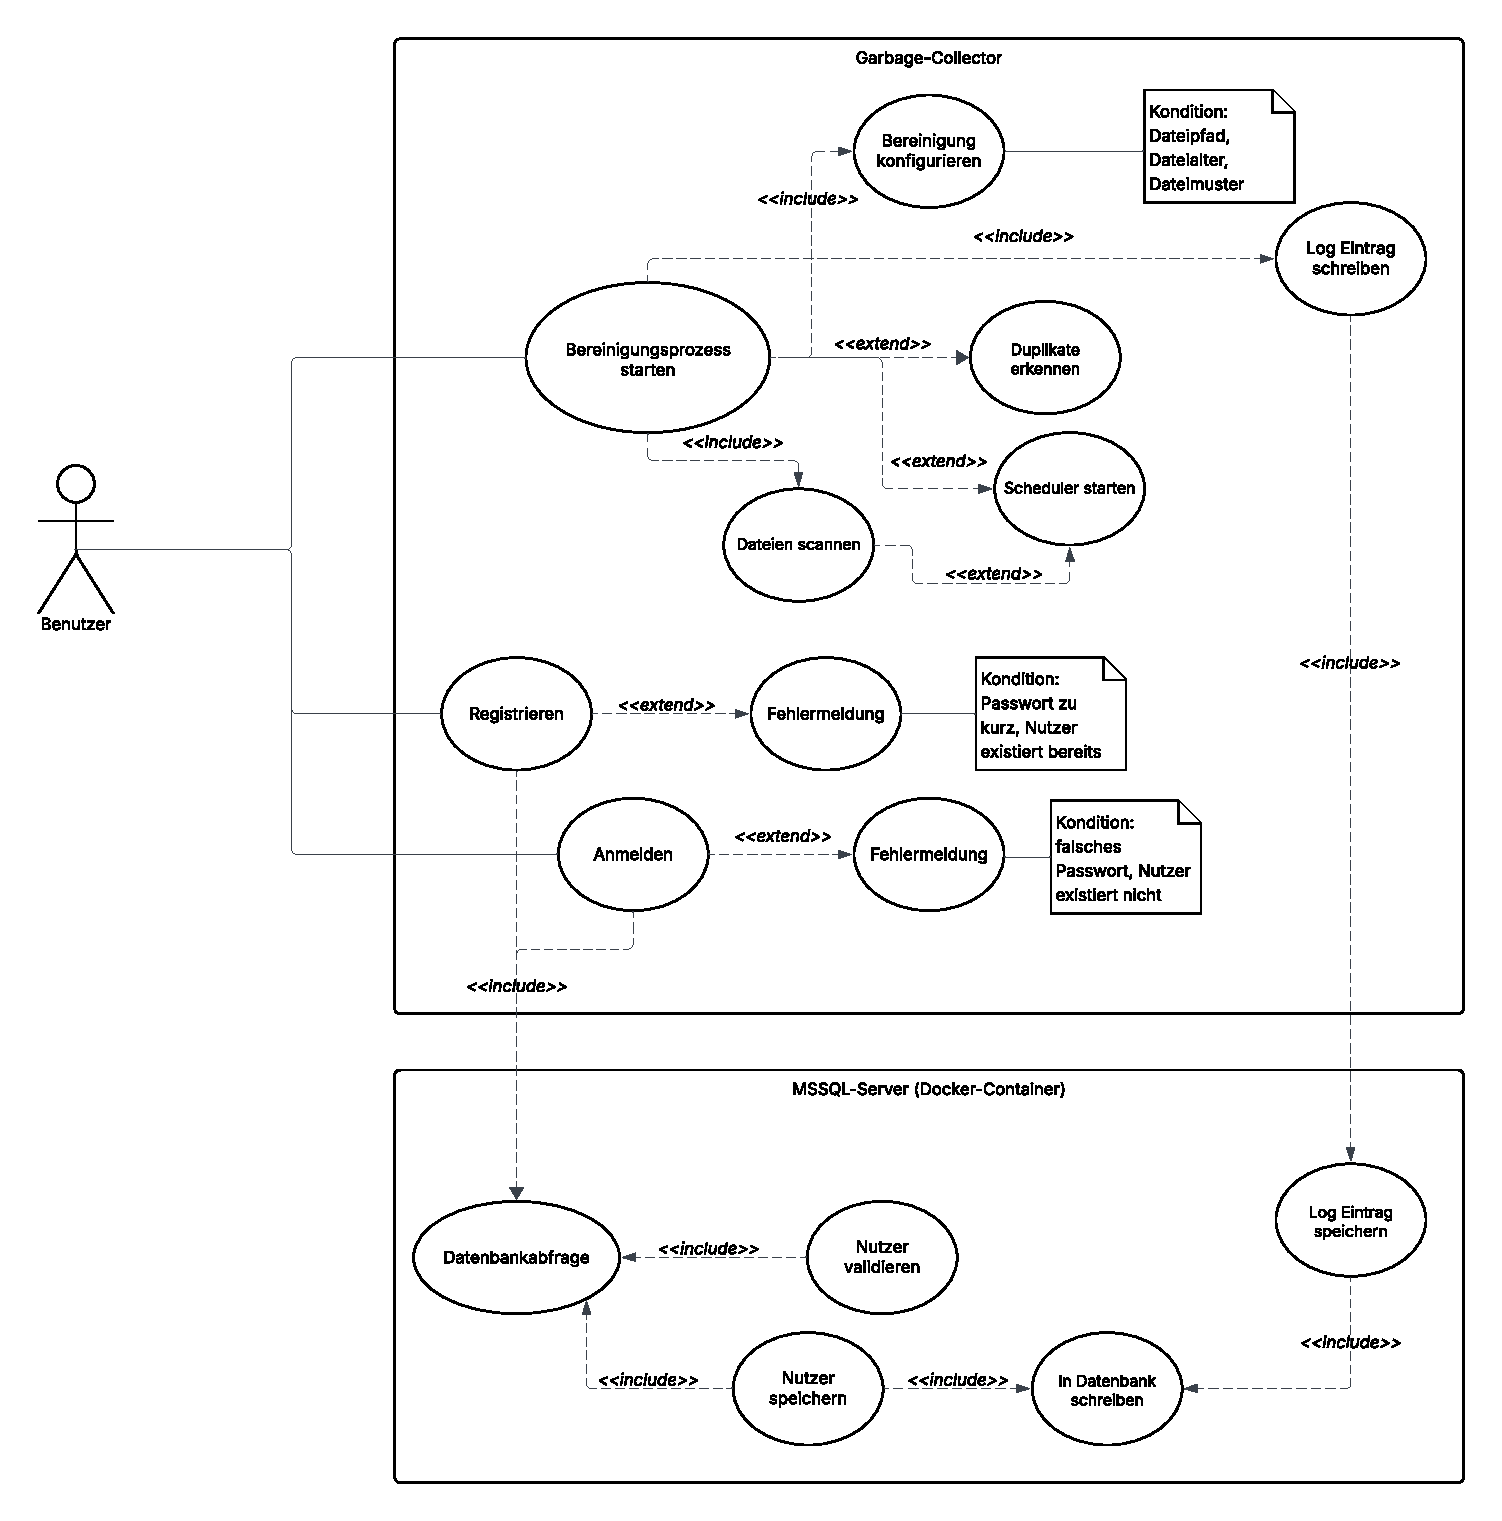
\includegraphics[width=\textwidth]{src/usecase_diagramm.pdf} 
    \caption{Use-Case-Diagramm des Garbage-Collection-Tools}
\end{figure}

\vspace{-0.5em}
\begin{footnotesize}
\textit{Hinweis: Das dargestellte Use-Case-Diagramm fokussiert sich auf die zentralen Anwendungsfälle des Garbage-Collection-Tools. Zusätzliche Funktionen wie Passwortänderung, Adminbereich oder weitere erweiterte Funktionen wurden aus Gründen der Übersichtlichkeit nicht aufgenommen und werden im weiteren Verlauf detaillierter beschrieben.}
\end{footnotesize}


\label{sec:usecases}

\subsubsection*{Use Case: Benutzer registrieren}
\begin{tabular}{|p{5cm}|p{10cm}|}
\hline
\textbf{Kurzbeschreibung} & Ein Benutzer erstellt ein neues Benutzerkonto im Garbage-Collector-Tool. \\
\hline
\textbf{Voraussetzung} & Der Benutzer ist noch nicht registriert. \\
\hline
\textbf{Nachbedingung} & Der Benutzer ist erfolgreich in der Datenbank gespeichert und kann sich künftig anmelden. \\
\hline
\textbf{Fehlersituation} & Das eingegebene Passwort ist zu kurz oder der Benutzername existiert bereits. \\
\hline
\textbf{Systemzustand im Fehlerfall} & Der Benutzer wird nicht registriert, eine Fehlermeldung wird angezeigt. \\
\hline
\textbf{Akteure} & Benutzer \\
\hline
\textbf{Trigger} & Der Benutzer klickt auf „Registrieren“ und füllt das Formular aus. \\
\hline
\textbf{Standardablauf} &
\begin{enumerate}
    \item Der Benutzer öffnet das Garbage-Collector-Tool.
    \item Der Benutzer klickt auf „Registrieren“.
    \item Das Tool prüft die Eingaben (z.\,B. Passwortlänge, eindeutiger Benutzername).
    \item Die Daten werden über eine Datenbankabfrage gespeichert.
    \item Der Benutzer erhält eine Bestätigung zur erfolgreichen Registrierung.
\end{enumerate}
\\
\hline
\textbf{Alternativabläufe} &
\begin{itemize}
    \item Das Passwort ist zu kurz.
    \item Der Benutzername ist bereits vergeben.
    \item Eine Fehlermeldung wird angezeigt und der Benutzer muss die Eingaben korrigieren.
\end{itemize}
\\
\hline
\end{tabular}


\subsubsection*{Use Case: Benutzer anmelden}
\begin{tabular}{|p{5cm}|p{10cm}|}
\hline
\textbf{Kurzbeschreibung} & Ein Benutzer meldet sich mit gültigen Zugangsdaten am System an. \\
\hline
\textbf{Voraussetzung} & Der Benutzer ist registriert und besitzt gültige Zugangsdaten. \\
\hline
\textbf{Nachbedingung} & Der Benutzer ist authentifiziert und erhält Zugriff auf die Funktionen der Software. \\
\hline
\textbf{Fehlersituation} & Das Passwort ist falsch oder der Benutzer existiert nicht. \\
\hline
\textbf{Systemzustand im Fehlerfall} & Keine Anmeldung, Zugriff wird verweigert, Fehlermeldung wird angezeigt. \\
\hline
\textbf{Akteure} & Benutzer \\
\hline
\textbf{Trigger} & Der Benutzer klickt auf „Anmelden“ und gibt Zugangsdaten ein. \\
\hline
\textbf{Standardablauf} &
\begin{enumerate}
    \item Der Benutzer öffnet das Tool und wählt „Anmelden“.
    \item Die Zugangsdaten werden über eine Datenbankabfrage geprüft.
    \item Die Anmeldung wird bestätigt.
    \item Der Benutzer hat Zugriff auf die Funktionen.
\end{enumerate}
\\
\hline
\textbf{Alternativabläufe} &
\begin{itemize}
    \item Falsches Passwort oder nicht existierender Benutzer.
    \item Fehlermeldung wird angezeigt, keine Anmeldung erfolgt.
\end{itemize}
\\
\hline
\end{tabular}

\vspace{1cm}

\subsubsection*{Use Case: Duplikate erkennen}
\begin{tabular}{|p{5cm}|p{10cm}|}
\hline
\textbf{Kurzbeschreibung} & Das Tool durchsucht die zu bereinigenden Dateien nach Duplikaten. \\
\hline
\textbf{Voraussetzung} & Die Bereinigung wurde gestartet. \\
\hline
\textbf{Nachbedingung} & Gefundene Duplikate werden zur weiteren Bearbeitung markiert oder entfernt. \\
\hline
\textbf{Fehlersituation} & Das System kann keine Duplikate erkennen (z.\,B. durch falsche Pfadangabe). \\
\hline
\textbf{Systemzustand im Fehlerfall} & Es werden keine Duplikate entfernt. \\
\hline
\textbf{Akteure} & Benutzer \\
\hline
\textbf{Trigger} & Der Benutzer startet die Bereinigung, das Duplikat-Erkennungsmodul wird automatisch aktiviert. \\
\hline
\textbf{Standardablauf} &
\begin{enumerate}
    \item Der Benutzer startet die Bereinigung.
    \item Das System durchsucht die angegebenen Verzeichnisse.
    \item Duplikate werden erkannt und entfernt oder dem Benutzer angezeigt.
    \item Ein Log-Eintrag wird erstellt.
\end{enumerate}
\\
\hline
\textbf{Alternativabläufe} &
\begin{itemize}
    \item Keine Duplikate gefunden.
    \item Das Duplikatmodul schlägt fehl, Log wird trotzdem erstellt.
\end{itemize}
\\
\hline
\end{tabular}

\vspace{1cm}

\subsubsection*{Use Case: Scheduler starten}
\begin{tabular}{|p{5cm}|p{10cm}|}
\hline
\textbf{Kurzbeschreibung} & Das Tool aktiviert eine Zeitsteuerung zur automatischen Durchführung von Bereinigungen. \\
\hline
\textbf{Voraussetzung} & Der Benutzer hat eine Konfiguration und den Zeitintervall festgelegt. \\
\hline
\textbf{Nachbedingung} & Der Scheduler ist aktiv und führt Bereinigungen gemäß Plan durch. \\
\hline
\textbf{Fehlersituation} & Es wurde kein oder ein falscher Pfad angegeben \\
\hline
\textbf{Systemzustand im Fehlerfall} & Keine automatische Bereinigung erfolgt. \\
\hline
\textbf{Akteure} & Benutzer \\
\hline
\textbf{Trigger} & Der Benutzer speichert eine Zeitsteuerung im Tool und startet den Scheduler. \\
\hline
\textbf{Standardablauf} &
\begin{enumerate}
    \item Der Benutzer öffnet die Einstellungen.
    \item Er konfiguriert einen automatischen Zeitplan.
    \item Der Benutzer aktiviert den internen Scheduler.
    \item Die geplanten Bereinigungen werden zum festgelegten Zeitintervall durchgeführt.
\end{enumerate}
\\
\hline
\textbf{Alternativabläufe} &
\begin{itemize}
    \item Ungültige Zeitangabe verhindert die Aktivierung.
    \item Fehlerhafte Konfiguration wird vom Tool gemeldet.
\end{itemize}
\\
\hline
\end{tabular}

\vspace{1cm}

\subsubsection*{Use Case: Log-Eintrag schreiben und speichern}
\begin{tabular}{|p{5cm}|p{10cm}|}
\hline
\textbf{Kurzbeschreibung} & Bei jedem Bereinigungsvorgang wird ein Log-Eintrag erstellt und in der Datenbank gespeichert. \\
\hline
\textbf{Voraussetzung} & Eine der drei Bereinigungstypen (Standard, Duplikate, Junk-Dateien)  oder Scheduler wurden ausgeführt \\
\hline
\textbf{Nachbedingung} & Ein entsprechender Eintrag befindet sich in der Log-Datenbank und steht zum Download bereit \\
\hline
\textbf{Fehlersituation} & Die Verbindung zur Datenbank ist unterbrochen oder Schreibrechte fehlen. \\
\hline
\textbf{Systemzustand im Fehlerfall} & Kein Eintrag in der Datenbank oder keine Verbindung \\
\hline
\textbf{Akteure} & (Internes Systemverhalten, ausgelöst durch Benutzeraktionen) \\
\hline
\textbf{Trigger} & Es wurde eine Bereinigung durch den Benutzer oder den Scheduler durchgeführt \\
\hline
\textbf{Standardablauf} &
\begin{enumerate}
    \item Eine Benutzeraktion (z.\,B. Start Bereinigung) wird ausgeführt.
    \item Das System erzeugt einen Log-Eintrag.
    \item Der Log-Eintrag wird an den MSSQL-Server weitergeleitet.
    \item Der Eintrag wird dauerhaft gespeichert.
\end{enumerate}
\\
\hline
\textbf{Alternativabläufe} &
\begin{itemize}
    \item Verbindung zur Datenbank schlägt fehl.
\end{itemize}
\\
\hline
\end{tabular}